\section{Berechnungen}

\subsection{Spielfeld}
\begin{figure}[h!]          
    \centering             
    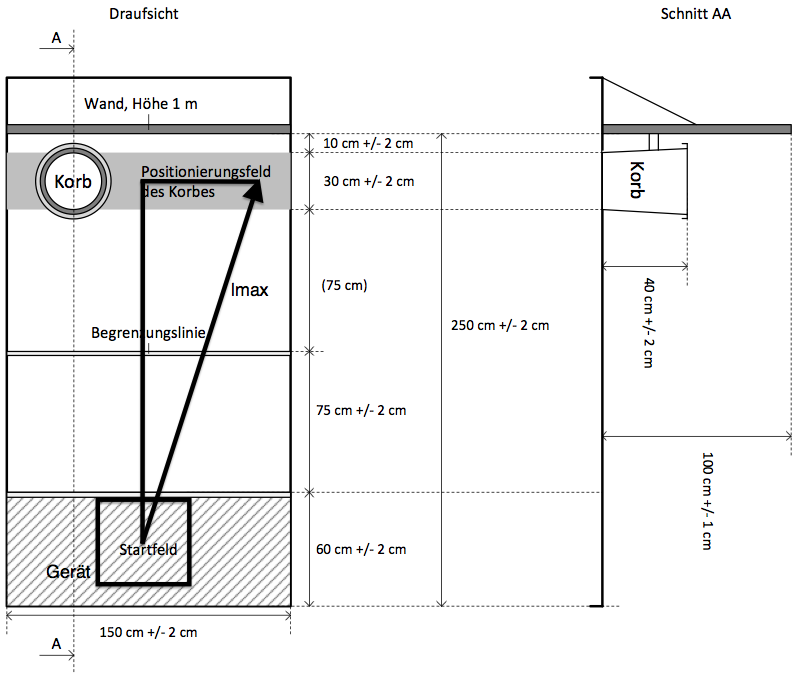
\includegraphics[width=0.8\textwidth]{fig/Bild_Spielfeld.png}    
    \caption{Spielfeld}
    \label{fig:spielfeld}        
\end{figure}
\noindent
Angenommen das Gerät wird im Startfeld mittig an der Startlinie positioniert, 
ausschliesslich mit einer drehbaren Abschussvorrichtung ausgerüstet, und der 
Korb ganz am Rand des Feldes positioniert, so ergibt sich für die maximale 
Wurflänge $l_{max}$ folgender Wert: 

\[\ l_\text{max} = \sqrt{(600mm)^2 + (1900mm)^2} = 1992.49mm \]

Somit ergibt sich im schlechtesten Fall ein Längenunterschied von ca 9.3 cm. 
Je nachdem wie hoch die Wurfgenauigkeit ist, könnte man die 9.3cm in 
Anbetracht des Korbdurchmessers von 30cm fast vernachlässigen, und ein 
Drehturm mit immer gleicher Wurflänge konstruieren. Voraussetzung ist, dass 
eine gute Zielgenauigkeit erreicht werden kann.

\subsection{Berechnungen Ballwurf}
Angenommen der Ball wird auf der Höhe des Korbes abgeworfen, kann mit 
folgender Formel berechnet werden, mit welcher Geschwindigkeit der Ball 
geworfen werden muss, falls er in einem Winkel $\alpha$ von 65$^\circ$ 
geworfen wird:
%
\[ v_0 
    = \sqrt{ \frac{s_x}{\sin(2 \cdot \alpha)} \cdot g } 
    = \sqrt{ \frac{1.9m}{\sin(2 \cdot 65^\circ)} \cdot 9.81 \frac{m}{s^2}} 
    = 4.93 \frac{m}{s} \]
%
Die maximale Höhe von 1.8 Metern darf nicht überschritten werden. Die Höhe 
die, der Ball erreicht lässt sich folgendermassen berechnen:
%
\[ h_\text{max} 
    = \frac{v_0^2 \cdot \sin(\alpha)^2}{2 \cdot g} 
    = \frac{4.93 \frac{m}{s}^2 \cdot \sin(65^\circ)^2}{2 \cdot 9.81 \frac{m}{s^2}} 
    = 1.018m \]
%
Die Zeit, die der Ball braucht, bis er im Korb ist, lässt sich folgendermassen 
berechnen:
%
\[ t = \frac{s_x}{v_0 \cdot \cos(\alpha)} 
    = \frac{1.9m}{4.93 \frac{m}{s} \cdot \cos(65^\circ)} = 0.911s \]
%
Nun werden die gleichen Rechnungen mit einem Winkel von 70$^\circ$ durchgeführt:
%
\[ v_0 = \sqrt{ \frac{s_x}{\sin(2\alpha)} \cdot g } 
    = \sqrt{ \frac{1.9m}{\sin(2 \cdot 70^\circ)} \cdot 9.81 \frac{m}{s^2}} 
    = 5.385 \frac{m}{s} \]

\[ h_\text{max} = \frac{v_0^2 \cdot \sin(\alpha)^2}{2 \cdot g} 
    = \frac{5.385 \frac{m}{s}^2 \cdot \sin(70^\circ)^2}{2 \cdot 9.81 \frac{m}{s^2}} 
    = 1.305m \]

\[ t = \frac{s_x}{v_0 \cdot \cos(\alpha)} 
    = \frac{1.9m}{5.385 \frac{m}{s} \cdot \cos(70^\circ)} = 1.032s \]
%
Wenn man davon ausgeht, dass es sich bei der Abschussgeschwindigkeit ein 
absoluter Fehler von $\pm$ 0.3 m/s einstellt, kann berechnet werden, mit 
welchem Winkel die Distanz mehr variiert:

\noindent
Winkel 65$^\circ$:
%
\[ s_x = \frac{(v_0 \pm \Delta v)^2 \cdot \sin(2 \cdot \alpha)}{g} 
    = \frac{(4.93 \frac{m}{s} \pm 0.3 \frac{m}{s})^2 \cdot \sin(2 \cdot 65^\circ)}{9.81 \frac{m}{s^2}} \]

\[ s_\text{xmax} = 2.136m \hspace{30mm} s_\text{xmin} = 1.674m \]
%
Winkel 70$^\circ$:
%
\[ s_x = \frac{(v_0 \pm \Delta v)^2 \cdot \sin(2 \cdot \alpha)}{g} 
    = \frac{(5.385 \frac{m}{s} \pm 0.3 \frac{m}{s})^2 \cdot \sin(2 \cdot 70^\circ)}{9.81 \frac{m}{s^2}} \]

\[ s_\text{xmax} = 2.118m \hspace{30mm} s_\text{xmin} = 1.694m \]
%
Bei einer Abschussgeschwindigkeitsänderung von lediglich $\pm$ 0.3m/s ergibt 
sich bereits eine Abweichung der Wurfweite von $\pm$ 20-25cm. Die 
Geschwindigkeit muss sehr genau eingestellt werden können und sehr konstant sein.

\noindent
Anhand dieser Berechnungen kann man auch sagen, dass die Längenänderung mit 
grösser werdendem Winkel kleiner wird. Somit wäre es besser, den Ball in einem 
grösseren Winkel zu schiessen. Allerdings muss dann der Ball schneller 
geschossen werden (mehr Energieaufwand, grösserer Rückstoss), der Weg wird 
länger und der Flug dauert länger.
